61. \begin{figure}[ht!]
\center{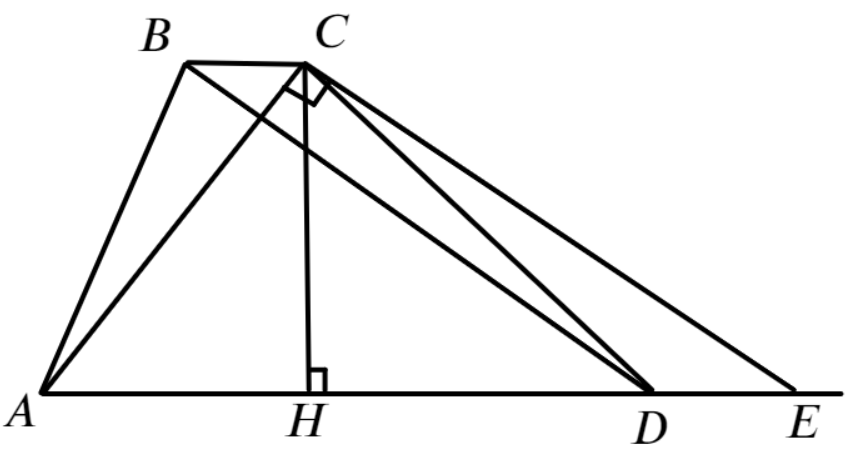
\includegraphics[scale=0.35]{g9-61.png}}
\end{figure}\\
Пусть диагональ $BD=5.$ Проведём через вершину $C$ прямую, параллельную $BD,$ точку её пересечения с прямой $AD$ обозначим буквой $E.$ Тогда $BCED$ является параллелограммом, а значит $CE=BD=5.$ Так как $AC\perp BD,$ то и $AC\perp CE.$ Опустим высоту $CH,$ тогда $HE=\sqrt{5^2-4^2}=3.$ Треугольники $ACH$ и $CHE$ подобны по двум углам ($\angle HCE=90^\circ-\angle HEC=\angle HAC,\ \angle CHE=90^\circ=\angle AHC$), значит $\cfrac{AC}{CE}=\cfrac{CH}{HK},\ \cfrac{AC}{5}=\cfrac{4}{3},\ AC=\cfrac{20}{3}.$ Тогда $S_{ABCD}=\cfrac{1}{2}CH\cdot(BC+AD)=\cfrac{1}{2}CH\cdot AE=S_{\Delta ACE}=\cfrac{AC\cdot CE}{2}=\cfrac{50}{3}.$\\
